%%%%%%%%%%%%%%%%%%%%%%%%%%%%%%%%%%%%%%%%%%%%%%%%%%%%%%%%%%%%%%%%%%%%%%%%%%%%%%%
% ISoIRS 2027 Full Paper  --  self-contained Overleaf project
%
% Upload the whole folder (or the zip) to Overleaf:
%   1. Overleaf -> New Project -> Upload Project -> choose isoirs_overleaf.zip
%   2. Set "main.tex" as the main document (it is usually detected automatically)
%   3. Recompile. IEEEtran ships with Overleaf; no extra packages to install.
%
% The layout reproduces the official ISoIRS Full Paper Template (IEEE two-column,
% A4, Times).  Compile order: pdflatex -> bibtex -> pdflatex -> pdflatex
%%%%%%%%%%%%%%%%%%%%%%%%%%%%%%%%%%%%%%%%%%%%%%%%%%%%%%%%%%%%%%%%%%%%%%%%%%%%%%%
\documentclass[conference]{IEEEtran}

\usepackage{cite}
\usepackage{amsmath,amssymb,amsfonts}
\usepackage{graphicx}
\usepackage{booktabs}
\usepackage{array}
\usepackage{url}
\usepackage[hidelinks]{hyperref}

\graphicspath{{figures/}}

\begin{document}

\title{Physical Consequence, Not Localization, Governs\\
Terrain-Induced Target Re-observability}

\author{
\IEEEauthorblockN{First Author, Second Author, Third Author}
\IEEEauthorblockA{Department, Organization\\
City, Country\\
first.author@example.edu}
}

\maketitle

\begin{abstract}
A robot that has already observed a target can lose sight of it because its own
motion and the intervening terrain block the line of sight. Restoring visibility is
not a search problem: the robot knows approximately where the target is, and that
knowledge is still not enough. This paper asks what information and what action
reasoning terrain-induced target re-observability actually requires, and answers by
elimination. Paired worlds that share terrain, pose, heading and a pixel-identical
current observation still require opposite re-observation actions, with disjoint
successful action sets in eight of eight pairs, so no memoryless rule can solve both;
a second family additionally shares the target memory and still requires different
optimal actions. Over 240 (state, action) pairs, 43.1\% of the actions a geometric
visibility oracle endorses fail when executed, while the same oracle placed at the
pose the robot actually reaches agrees with the physical outcome 97.9\% of the time,
so the missing quantity is the physical consequence of an action rather than its
visibility. On 2240 physically executed (state, action) pairs, adding the candidate
action to observation plus memory raises re-observation AUC from 0.854 to 0.934,
whereas adding the current observation to the memory buys 0.002. A planner built on
the resulting action-conditioned consequence model reaches RSR@10 of 0.792 without
privileged information, against 0.625 for uninformed random choice and 0.250 for every
classical rule, while using 36 percent less motion than random choice. Three negative results
bound how such a model may be used. Anchor recovery under perfect localization still
fails physically in six of twenty-four terrains. A safety consequence head that is
accurate and made better calibrated exactly where the decision threshold acts yields
zero planning gain. Lookahead of two, three and five steps is not significantly
better than one step on any budget while costing 1.8 to 2.1 times the motion. All
results are in simulation with a vendored third-party locomotion policy; we claim the
formulation, the benchmark, the failure analysis and the identification of the
missing quantity, not a world model.
\end{abstract}

\begin{IEEEkeywords}
target re-observability, terrain-induced occlusion, action-conditioned consequence
prediction, partial observability, legged locomotion, benchmark, failure analysis
\end{IEEEkeywords}

\section{Introduction}

Robots operating in natural terrain rarely enjoy a clear view of what they care
about. A legged platform descending into a crater, a rover traversing a ridge line, or
a manipulator reaching behind a boulder all face the same structural problem: the
terrain determines what can be seen from where, and the robot's own motion is what
changes it. Partial observability here is not sensor noise but a deterministic
consequence of geometry, and therefore predictable in principle --- but only if the
robot reasons about how its next action will change what it can see.

This paper studies a specific instance of that problem. The robot has already
observed a target. Later the target is no longer visible, not because it moved or the
sensor failed, but because the robot's own position and the intervening terrain now
block the line of sight. The robot must choose an action that makes the target visible
again. We call this \emph{target re-observability}, and it differs from classical
search in one decisive way: the robot has information about where the target is, and
that information is still not enough.

The natural intuition that moving toward a target makes it more likely to be seen
fails under terrain. Measured along a traverse toward a target beyond a ridge, the
visibility sequence is not a single transition from visible to hidden but alternates:

\begin{center}
\small
\begin{tabular}{llll}
\toprule
terrain & profile & terrain & profile\\
\midrule
\texttt{stairs\_up}   & V X V X   & \texttt{waves}        & X V X V X\\
\texttt{trench}       & V X V X   & \texttt{perlin}       & X V X V X\\
\texttt{pit}          & V X V X   & \texttt{basin}        & X V X\\
\texttt{barrier}      & V X V X   & \texttt{perlin\_rough}& X V X V X\\
\bottomrule
\end{tabular}
\end{center}

\noindent where V marks a position from which the target is visible and X one from
which it is blocked. The number of transitions ranges from two to four on a single
traverse. A policy that assumes monotonicity is not merely imprecise; it is aimed at
the wrong objective.

Prior work supplies necessary components but addresses different questions.
Lost-target search maintains a belief over where the target went and selects search
actions to reduce it \cite{RadmardCroft2016,Radmard2018}. Occlusion-aware active
perception and next-best-view select viewpoints by predicting visibility or
information gain from a candidate pose, typically using geometry rather than execution
\cite{OANBV,LEAPNBV}. Object permanence filters maintain a belief through periods of
non-observation \cite{Peng2024}. Embodied visual tracking and target-loss recovery is
an established direction with its own benchmarks and systems
\cite{TrackVLA,EVTBench}, and work in that line already combines action-conditioned
world models with model-predictive control for recovering a lost target
\cite{CSTWM}, while recent work couples visibility with reachability and feasibility
\cite{VisibleReachable}. None of this is unstudied, and we do not claim otherwise.
What is missing is a unified analysis: these lines are evaluated in their own
settings, with their own observation and action interfaces and their own budgets, so
the boundaries between them are not visible. We place the same decision rules on one
task --- terrain fixed, target static, action set identical, only the decision rule
differing --- and ask where and why each breaks.

This paper makes the following contributions. First, a formulation of terrain-induced
target re-observability as an action-selection problem, with the non-monotonicity of
visibility along a traverse as its defining property. Second, a procedurally generated
benchmark of eight terrain-induced occlusion mechanisms, organised by physical
mechanism and real-world analogue rather than as a difficulty ladder, with paired
worlds that are provably identical in the current observation. Third, a frozen
observation and action interface under which every decision rule is evaluated on the
same terrain, budget and termination set, with all comparisons reported as paired
bootstrap intervals. Fourth, a measured identification of the missing quantity,
together with three negative results showing that accurate prediction is not the same
thing as decision usefulness.

\section{Related Work}

Lost-target search maintains a belief over target location and plans search actions to
reduce uncertainty \cite{RadmardCroft2016,Radmard2018}. It answers which search action
best reduces uncertainty, but not what to do when terrain makes the correct
re-observation action point away from the belief. In our paired worlds the belief is
correct and the action that restores visibility lies on the opposite side.

Occlusion-aware active perception and next-best-view score candidate viewpoints by
predicted visibility or information gain \cite{OANBV,LEAPNBV}. Candidate poses are
typically evaluated kinematically, which assumes that an action takes the robot
exactly where its nominal displacement says. We measure that this assumption fails,
and that the visibility model itself is not the problem.

Object permanence maintains a belief through non-observation and acts on the filtered
estimate \cite{Peng2024}. It answers where the target probably is; it does not
establish that knowing where the target is determines what to do. Our second pair
family isolates exactly that gap.

Embodied visual tracking and target-loss recovery is an established direction
\cite{TrackVLA,EVTBench}, with work already combining action-conditioned world models
and model-predictive control for target recovery \cite{CSTWM}, and recent work
coupling visibility with reachability and feasibility \cite{VisibleReachable}. Our
focus is narrower and physical: which quantity must be predicted for a known target to
be made visible again under terrain-induced occlusion, and how that prediction should
enter a decision.

\section{Problem Formulation}

Let $O_t$ be the observation at time $t$, comprising pose, proprioception and a short
action history; $M_t$ the target memory, that is where and when the target was last
seen; and $a_{t:t+H}$ a sequence of physical actions. Write $V_{t+h} \in \{0,1\}$ for
target visibility after executing that sequence. The task is

\begin{equation}
a^{*}_{t:t+H} \;=\; \operatorname*{arg\,max}_{a_{t:t+H}}\;
P\!\left(V_{t+H}=1 \mid O_t, M_t, a_{t:t+H}\right)
\label{eq:objective}
\end{equation}

\noindent The target is \emph{lost} when $V_t = 0$ after having been observed, and
\emph{re-observed} when there exists $h \le H$ with $V_{t+h} = 1$. Physical safety is
deliberately not part of this definition: Section~\ref{sec:discussion} shows that
safety is a dimension of the consequence model rather than part of the task statement,
and mixing it into \eqref{eq:objective} would confound the two.

The benchmark reports a difficulty curve rather than a single success flag, because
the quantity of interest is how many physical actions are needed to regain sight. For
episode $i$ and budget $K$,

\begin{equation}
r_i(K) = \mathbf{1}\!\left[\exists\, h \le K : V_{i,t+h} = 1\right],
\qquad
\mathrm{RSR}@K = \frac{1}{N}\sum_{i=1}^{N} r_i(K)
\label{eq:rsr}
\end{equation}

\noindent Note what the definition does not require: visibility to be held.
Visibility under these mechanisms is non-monotonic, and the task is to regain sight
within a budget, not to keep it. The implementation is audited against
\eqref{eq:rsr} rather than assumed to match it: the metric is evaluated directly on
the recorded per-step visibility trace, and a contract test asserts that this agrees
with reading the termination state, so the headline number cannot drift if the episode
semantics change.

Two companion metrics are reported and no single scalar combines them. The
re-observation time $T_{\mathrm{reobs}}$ is the elapsed time from loss to the first
re-observation. The action cost $C_{\mathrm{action}}$ is cumulative base-path length,
averaged over every episode rather than only the successful ones so that exhausting
the budget does not look cheap.

\section{Method}

\subsection{Visibility State and the Missing Quantity}

H1, H2 and H3 below remove the simple explanations one at a time: the current
observation does not determine the action, a correct target memory does not determine
it either, and geometric visibility does not predict physical re-observation. The
quantity that remains is the action-conditioned physical consequence. Rather than
learning visibility end to end, we exploit the third result: since the visibility
oracle is accurate at whatever pose the robot actually reaches, the model predicts the
executed body-frame pose delta and the already-validated oracle is applied to the
predicted pose. This keeps the validated part validated and localises the remaining
error.

\subsection{Candidate Actions and the Consequence Model}

Candidate actions are ten fixed locomotion primitives, each of the same simulated
duration so that one step is one unit of budget. The consequence model is trained on
2240 physically executed (state, action) pairs, that is 24 terrains by 10 states by 10
actions, with positive rate 0.143. Features are the pose, the projected gravity
vector, a short pose history, the target memory expressed in body coordinates with an
explicit presence flag, and the action. Targets are the executed pose delta and
whether the target was re-observed. Splits are by terrain and never random, so a
terrain family cannot appear on both sides.

\subsection{Closed-Loop Action Selection}

The planner scores every candidate action with the model, takes the argmax of the
predicted re-observation probability, and replans after each executed step, giving a
receding-horizon controller over the learned model. An episode terminates at the first
re-observation, at a fall, or on leaving the terrain.

\section{Experimental Setup}

\subsection{Benchmark}

The suite comprises eight terrain-induced occlusion mechanisms, listed in
Table~\ref{tab:mechanisms} and organised by physical mechanism rather than by surface
name. Each is a situation in which a robot that has already seen a target loses sight
of it and must regain sight by moving. The mechanisms span five roughly orthogonal
axes: occlusion direction, elevation dependence, spatial scale, visibility transition
frequency, and terrain spatial complexity. A mechanism is a point on an axis rather
than a member of a category: \texttt{pit} and \texttt{basin} are both spatial scale,
at opposite ends of it.

\begin{table}[t]
\caption{Terrain-induced occlusion mechanisms. A mechanism is a point on an axis, not
a member of a category.}
\label{tab:mechanisms}
\centering
\small
\begin{tabular}{@{}lll@{}}
\toprule
Mechanism & Axis & Real-world analogue\\
\midrule
\texttt{barrier}       & occlusion direction & walls, boulders, shelving\\
\texttt{trench}        & elevation           & ditches, trenches, ravines\\
\texttt{stairs\_up}    & elevation           & staircases, platforms\\
\texttt{pit}           & spatial scale       & potholes, craters\\
\texttt{basin}         & spatial scale       & valleys, depressions\\
\texttt{waves}         & visibility dynamics & dunes, rolling ground\\
\texttt{perlin}        & terrain complexity  & natural off-road ground\\
\texttt{perlin\_rough} & terrain complexity  & rubble, rock fields\\
\bottomrule
\end{tabular}
\end{table}

Two framing rules are enforced mechanically rather than left to intent. The taxonomy
is checked for the wording \emph{challenging}, \emph{hard}, \emph{difficult} or
\emph{adversarial terrain} and refuses to render if it appears, because the difficulty
is in the target's visibility and not in the driving. And \texttt{perlin} and
\texttt{perlin\_rough} are not claimed to be real surfaces: Perlin noise is used as a
procedural representation of spatially correlated natural elevation variation. All
terrain is built as explicit box slabs rather than as a height field, so that the
analytic visibility oracle and the collision surface are the same object.

\subsection{Baselines and Metrics}

Every baseline implements the core decision mechanism of a line of work rather than a
full reproduction. \textsc{Reactive} always drives forward. \textsc{HeadingLock} holds
the heading recorded at the loss moment. \textsc{HistoryOnly} aims at the remembered
target. \textsc{LostTargetSearch} faces the belief and closes on it.
\textsc{ObjectPermanence} runs a constant-velocity belief filter. \textsc{NBV}
re-projects the believed target from a kinematic pose and is given the exact height
field, since an active-perception method is allowed a map. \textsc{Random} draws
uniformly from the frozen action set and establishes the lower bound.
\textsc{Oracle} physically rolls out every candidate and is a privileged upper bound,
never a deployable method.

Metrics are $\mathrm{RSR}@K$ as defined in \eqref{eq:rsr}, $T_{\mathrm{reobs}}$, and
$C_{\mathrm{action}}$. Every proportion carries a Wilson score interval rather than a
normal approximation, because several results sit at or near zero or one. Every
comparison is paired: since all policies run on the same terrains, a difference in
$\mathrm{RSR}$ is tested by resampling terrains with replacement and examining the
distribution of the paired difference.

\section{Results}

\subsection{The Current Observation Does Not Determine the Action}

We construct paired worlds that share terrain, robot pose, heading and a
pixel-identical current observation, but in which the target was last seen from
opposite sides. Across eight pairs the rendered camera images are identical with mean
and maximum absolute pixel difference both zero, the optimal re-observation action is
opposite in the two worlds in eight of eight, and the successful action sets are
disjoint in eight of eight. Because any function of the current observation takes the
same value in both worlds, no memoryless policy can solve both. On sixteen
paired-history worlds the five classical rules score zero of sixteen.

\subsection{A Correct Target Memory Is Also Not Sufficient}

A natural reply is to remember where the target is. We therefore construct a second
family of pairs sharing the current observation and the reconstructed target memory,
differing only in terrain hidden inside the shadow of a visible occluder, which is
invisible from the decision point and was never traversed. Over six such pairs the
rendered observations are pixel-identical in six of six, the target memory is
identical in six of six, and the optimal action differs in four of six. Two properties
bound the claim. The successful action sets overlap, so this does not show that no
fixed rule can succeed; it shows that a correct memory does not determine the optimal
action. And on these pairs all six classical policies choose the same action and fail
in both worlds, so the construction is an information-level result and not a
behavioural one.

\subsection{Geometric Visibility Is Not Physical Re-observability}

For every candidate action at every decision state we compute two quantities.
$G(s,a)$ asks whether the target would be visible if the robot reached the ideal pose
the action nominally produces, using a kinematic displacement and the line-of-sight
oracle. $P(s,a)$ asks whether the target is actually re-observed when the primitive is
executed. Over 240 pairs, the confusion matrix is $(G{=}0,P{=}0)=171$,
$(G{=}0,P{=}1)=11$, $(G{=}1,P{=}0)=25$ and $(G{=}1,P{=}1)=33$. That is, $43.1\%$ of
the actions geometry endorses fail physically, and the disagreement is not
one-sided: geometry also under-predicts in $4.6\%$ of cases. Placing the same oracle
at the pose the robot actually reaches makes it agree with the physical outcome in
$97.9\%$ of pairs. The pose prediction error is larger on the failing cell than on the
agreeing cells by a paired bootstrap difference of $+0.28$\,m with a $95\%$ interval
of $[+0.11, +0.45]$\,m, decomposed into $0.52$\,m forward, $0.34$\,m lateral,
$0.40$\,m in height and $5.5$ degrees of yaw. No active-perception method is
mis-implemented here; candidate viewpoints scored kinematically are simply a different
quantity from where the robot ends up.

\subsection{Information Ablation}

Table~\ref{tab:ablation} ablates the predictor input with terrain held out. Adding the
candidate action raises AUC by $+0.080$, while adding the current observation to the
memory raises it by $+0.002$. The information is in the action, not in seeing more. On
the sixteen paired-world decision states the model reaches $0.81$ accuracy and
switches its chosen action in eight of eight pairs, which is what a memoryless rule
provably cannot do.

\begin{table}[t]
\caption{Information ablation, leave-one-terrain-out, 2240 samples. Scores are
ROC-AUC; pose error is mean absolute error over the four body-frame components. Best
in bold.}
\label{tab:ablation}
\centering
\small
\begin{tabular}{@{}lccccc@{}}
\toprule
Inputs & ROC-AUC & PR-AUC & Brier & ECE & Pose MAE (m)\\
\midrule
$O$            & 0.759 & 0.360 & 0.117 & 0.076 & 0.436\\
$M$            & 0.852 & 0.639 & 0.077 & 0.039 & 0.461\\
$O{+}M$        & 0.854 & 0.600 & 0.084 & 0.056 & 0.425\\
$O{+}M{+}a$    & \textbf{0.934} & \textbf{0.748} & \textbf{0.062} &
                 \textbf{0.022} & \textbf{0.148}\\
\bottomrule
\end{tabular}
\end{table}

\subsection{Analytic Versus Learned Consequence}

The learned pose model is compared against the analytic nominal displacement, which is
what a kinematic predictor assumes. Mean absolute error falls from $0.469$ to
$0.148$, a factor of $3.2$, with per-component ratios of $5.5$ for forward, $2.9$ for
lateral and $3.7$ for yaw. The analytic model is nevertheless better for height, at
$0.090$ against $0.149$, because it predicts no change and changes are small. The
correct statement is that the learned model wins on the components that decide
success, not that learning is better in all dimensions.

\subsection{Consequence Prediction Converts Into Task Performance}

Table~\ref{tab:main} reports the multi-step protocol over 24 terrains with identical
budget and termination set for every method. The consequence planner reaches
$\mathrm{RSR}@10 = 0.792$ and $\mathrm{RSR}@1 = 0.708$ with no privileged information,
against $0.625$ for \textsc{Random} at $1.6$ times the motion cost. By contrast, no
classical baseline significantly outperforms any other: relative to
\textsc{HistoryOnly}, \textsc{Reactive}, \textsc{HeadingLock},
\textsc{LostTargetSearch} and \textsc{ObjectPermanence} each differ by $0.000$ with
interval $[0,0]$, that is, they succeed and fail on exactly the same terrain set.
\textsc{NBV} differs by $+0.042$ with interval $[0.00, 0.125]$ and $p = 0.356$, so it
cannot be claimed to be better. Only the privileged references separate.

\begin{table}[t]
\caption{Multi-step episode protocol, 24 terrains, budget $10 \times 3.0$\,s. Every
method uses the same action set, budget and termination set. Success is the
re-observation rate; cost is mean base-path length over all episodes. Best non
privileged result in bold.}
\label{tab:main}
\centering
\small
\begin{tabular}{@{}lcccc@{}}
\toprule
Method & RSR@1 & RSR@3 & RSR@5 & RSR@10\\
\midrule
\textsc{Random} (lower bound)      & 0.083 & 0.542 & 0.625 & 0.625\\
\textsc{Reactive} / \textsc{HeadingLock} / \textsc{HistoryOnly}
                                   & 0.167 & 0.250 & 0.250 & 0.250\\
\textsc{NBV}                       & 0.167 & 0.208 & 0.250 & 0.250\\
\textsc{Anchor recovery} (perfect) & 0.167 & 0.250 & 0.250 & 0.250\\
\textbf{Consequence planner (ours)} & \textbf{0.708} & \textbf{0.708} &
                                     \textbf{0.792} & \textbf{0.792}\\
\midrule
\textsc{Oracle} (privileged)       & 0.833 & 0.875 & 0.875 & 0.875\\
\textsc{Oracle search} (privileged)& 0.750 & 1.000 & 1.000 & 1.000\\
\bottomrule
\end{tabular}
\end{table}

\begin{figure}[t]
\centering
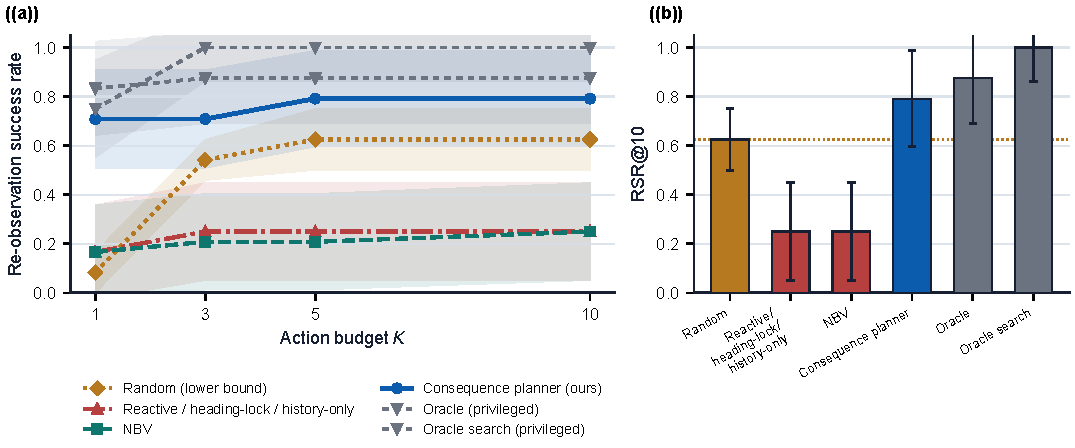
\includegraphics[width=\columnwidth]{fig_main.pdf}
\caption{Re-observation performance and the baseline ladder, over 24 terrains with a
10-step budget. (a) Success rate against action budget; intervals are Wilson $95\%$
intervals, except for \textsc{Random}, which is a mean over three seeds and whose band
is the spread across those seeds. (b) Success at the full budget with Wilson $95\%$
intervals. \textsc{Random}, which never commits to a single action, sits above every
classical rule; the consequence planner is higher still, at lower motion cost. The
privileged oracles are reference bounds and are not deployable methods.}
\label{fig:main}
\end{figure}

\subsection{Cross-Mechanism Generalisation}

The unit of generalisation here is the mechanism, not the terrain. An earlier
predictor held out a single terrain, which for the sixteen paired-history worlds still
leaves fifteen members of the same mechanism in training; that measures
within-mechanism generalisation and cannot answer this question. We therefore hold out
an entire mechanism family at once. The learned pose model beats the analytic baseline
on all five held-out mechanisms, at a mean error of $0.329$ against $0.491$, so the
causal structure from action to future physical state does transfer. Accuracy
nevertheless degrades relative to the within-mechanism reference, where mean pose
error is $0.196$ and mean AUC $0.897$ against $0.810$ across mechanisms. The
occlusion-direction fold reaches an AUC of $0.533$, but that fold also removes 1680 of
2240 training rows, so it confounds the mechanism shift with a large reduction in data
and cannot be attributed to mechanism transfer alone.

\section{Failure Analysis and Discussion}
\label{sec:discussion}

\subsection{The Task Is Not Localisation Recovery}

The most damaging reading of this benchmark is that it reduces to state recovery:
save the pose at which the target was last seen and use odometry to return to it. We
implement three such baselines --- steering back to the last-visible pose,
dead-reckoned backtracking along the recorded walk-in, and returning to that pose
before advancing along the original sight ray --- under perfect, moderate and
realistic odometry drift. Perfect odometry does not solve the task: the best
anchor-recovery baseline reaches $\mathrm{RSR}@10 = 0.250$, the same as the classical
rules and far below the consequence planner. More pointedly, six of its twenty-four
failures under perfect localisation are physical terminations, meaning the robot falls
or leaves the terrain while returning to a pose it knows exactly. Perfect and moderate
drift produce identical results and realistic drift changes $\mathrm{RSR}@10$ by
$0.000$, so the failure is not an odometry-accuracy problem but the physical
consequence gap reached from an independent direction. Knowing exactly where the robot
was does not imply that re-observation is physically executable.

\subsection{Failure Type Changes With Planner Capability}

Table~\ref{tab:taxonomy} classifies failures. Classical policies predominantly fail
because they select ineffective actions, whereas the learned consequence planner
substantially reduces action-selection failures and instead exposes physical
termination failures. This shift is itself evidence that the modelled quantity is the
right one and that the remaining gap concerns the coverage of the consequence model
rather than candidate diversity. Our first version of this taxonomy recorded falls and
boundary exits as action-selection failures, which is an attribution error: the action
was chosen on a defensible prediction and what failed was the prediction of
stability.

\begin{table}[t]
\caption{Failure classification under protocol B, 24 terrains. $B$: belief present and
a good action existed but was not chosen. $F$: the action was selected from a
defensible prediction and the physical outcome was not anticipated.}
\label{tab:taxonomy}
\centering
\small
\begin{tabular}{@{}lccc@{}}
\toprule
Planner & $B$ action & $F$ termination & Other\\
\midrule
\textsc{HeadingLock} / \textsc{HistoryOnly} / \textsc{LostTargetSearch} /
  \textsc{ObjectPermanence} & 18 & 0 & ---\\
\textsc{Reactive}      & 17 & 1 & ---\\
\textsc{NBV}           & 16 & 1 & $C$ 1, $D$ 1\\
\textbf{Consequence planner} & \textbf{1} & \textbf{4} & ---\\
\textsc{Oracle}        & 3 & 0 & ---\\
\bottomrule
\end{tabular}
\end{table}

\subsection{Better Prediction Is Not Better Decisions}

Two negative results bound how a consequence model may be used, and both concern the
prediction-to-decision step rather than prediction quality. Adding a safety
consequence head raises the privileged oracle with ground truth from $0.3884$ to
$0.4107$, so the term is worth having, and the learned head is accurate with
ROC-AUC $0.900$. Yet the planner gets worse at every penalty weight. Fixing the
obvious explanation does not help: the head's overall calibration error is $0.042$
while its error in the band where a threshold actually acts is $0.197$, a factor of
$4.7$, and temperature scaling halves that to $0.099$ and produces exactly zero
planning improvement. Across raw, temperature-scaled and isotonic variants no
operating point at any threshold or coverage beats not using safety at all.

A dependence analysis over the same 2240 samples explains why. Visibility and safety
are negatively coupled, with an odds ratio of $0.35$ and a $95\%$ interval of
$[0.249, 0.492]$, so the actions that reveal the target are less safe than those that
do not, and the coupling persists within six of the ten individual actions, so it is
not merely induced by action choice. But it almost never creates a decision conflict:
safe actions are abundant at $9.17$ per state and visible actions scarce at $1.43$,
and only five of 224 states have a visible action and a safe action but none that is
both. The headroom for any joint decision is therefore bounded by that $2.2\%$
conflict set, which is smaller than the noise in any learned head, and the joint head,
a product of the two marginals, and a conformal filter all fail to improve on the
visibility-only planner.

Longer lookahead fails in the same shape. Intermediate states in a chained rollout
come from the learned model and never from ground-truth stepping, and only the first
action of each plan is executed. Against a horizon of one step, paired success
differences are $-0.208$ with interval $[-0.458, 0.042]$, $0.000$ with
$[-0.208, 0.208]$, and $-0.125$ with $[-0.333, 0.083]$ for horizons of two, three and
five. No horizon is significantly better on any budget, and every horizon costs $1.78$
to $2.09$ times the motion. Lookahead does rescue two terrains that genuinely require
multiple steps, which confirms that re-observation is intrinsically sequential, but it
breaks eight terrains that one step solves. Model-error accumulation is not the
explanation: the measured one-step pose error is lowest at a horizon of two and that
horizon performs worst. The mechanism is that a chained score taking a maximum over
steps is monotonically optimistic in the horizon, so a longer lookahead offers more
opportunities to find a sequence the model confidently believes will glimpse the
target, and those are precisely the confidently wrong predictions. Longer rollout is
not automatically beneficial when consequence uncertainty accumulates.

\subsection{Limitations}

All results are from simulation with a vendored third-party locomotion policy on a
single controller, and no sim-to-real claim is made. The oracle is a privileged upper
bound and the search reference is incomplete: an earlier version of this work judged
four terrains unsolvable and beam search subsequently solved all four with two- to
three-step sequences, so mistaking a planner's defect for a property of the benchmark
nearly put a spurious ceiling into the results. The learned consequence model is
evaluated with terrain held out, which is generalisation within a mechanism family.
The target memory is a structured location representation reconstructed without noise,
so belief-estimation failure is excluded by construction. The action set is ten fixed
primitives and whether discretisation affects the paired-world conclusions has not
been tested. A binary fall label proved unusable, with zero falls in 720 single-action
rollouts, so stability is represented by boundary exit and a continuous margin, which
means the learned safety head does not cover the event it is named after. Finally, the
paired-world construction is available only in mechanisms that can express a
directional aperture; five mechanisms where this is structurally impossible are
documented in the benchmark definition.

\section{Conclusion}

We asked what information and what action reasoning a robot needs in order to regain
sight of a target that terrain has occluded. The current observation is not
sufficient, because worlds with pixel-identical observations can require opposite
actions with disjoint successful sets. A correct target memory is not sufficient
either, because worlds identical in observation and in memory can still require
different actions. Geometric visibility is not sufficient, because $43.1\%$ of the
actions it endorses fail physically while the same oracle at the executed pose agrees
with physics $97.9\%$ of the time. What is missing is the action-conditioned physical
consequence: adding the candidate action to observation plus memory raises predictive
AUC by $0.080$ while adding the observation to the memory raises it by $0.002$, and a
planner built on the resulting model reaches $\mathrm{RSR}@10 = 0.792$ without
privileged information, against $0.625$ for uninformed random choice and $0.250$ for
every classical rule, while using $36\%$ less motion than random choice.

Three negative results bound how such a model may be used, and all concern the
prediction-to-decision step rather than prediction quality. Perfect localisation does
not guarantee physical re-observability. A safety head that is accurate and made
better calibrated at the decision boundary produces zero planning gain. Deeper
lookahead is not significantly better on any budget, costs nearly twice the motion,
and rescues two genuinely sequential terrains while breaking eight that one step
solves. The compact statement of the paper is therefore that observation plus memory
does not imply the optimal action, and the reason is the step in between: action to
future physical state to future visibility must be modelled explicitly, must be
action-conditioned, and must then be turned into a decision rather than a threshold.

\bibliographystyle{IEEEtran}
\bibliography{references}

\end{document}
